\documentclass[11pt]{article}
\usepackage[margin=1in]{geometry}
\usepackage{fontspec}
\usepackage{booktabs}
\usepackage{array}
\usepackage{float}
\usepackage{graphicx}
\usepackage{adjustbox}
\usepackage{amsmath}
\usepackage[font=small,labelfont=bf]{caption}
\usepackage{natbib}
\usepackage{xurl}
\usepackage[hidelinks]{hyperref}
\usepackage{setspace}
\setstretch{1.15}
\graphicspath{{../figs/}}
\newcommand{\nStudyOne}{382}
\newcommand{\nStudyTwo}{596}
\newcommand{\nTiming}{284}
\newcommand{\nWording}{312}
\newcommand{\sumEffect}{-0.5}
\newcommand{\standardBias}{18.9}
\newcommand{\sumBias}{18.4}
\newcommand{\sumBlackAbs}{7.8}
\newcommand{\sumSouth}{18.6}
\newcommand{\sumSouthMean}{60.9}
\newcommand{\standardSouthMean}{42.3}
\newcommand{\incEffect}{0.9}
\newcommand{\incLo}{-3.6}
\newcommand{\incHi}{5.3}
\newcommand{\brEffect}{7.2}
\newcommand{\brLo}{2.2}
\newcommand{\brHi}{12.1}
\newcommand{\brItemsUp}{all eight}
\newcommand{\timeEffect}{4.3}
\newcommand{\timeLo}{1.5}
\newcommand{\timeHi}{7.1}
\newcommand{\fastBias}{19.8}
\newcommand{\slowBias}{15.6}
\newcommand{\timeDecline}{22}
\newcommand{\timeItemsLower}{ten}
\newcommand{\timeItemsFive}{three}
\newcommand{\timeItemsTen}{five}
\newcommand{\timePoorDiff}{0.05}
\newcommand{\wordEffect}{1.2}
\newcommand{\wordLo}{-3.7}
\newcommand{\wordHi}{1.2}
\newcommand{\hundredBias}{19.1}
\newcommand{\percentBias}{17.7}
\newcommand{\hundredLowerItems}{three}
\newcommand{\wordImm}{6.1}
\newcommand{\wordLgb}{5.3}
\newcommand{\slowPages}{1,223}
\newcommand{\slowUnder}{8}
\newcommand{\slowMedian}{17.0}
\newcommand{\fastPages}{1,210}
\newcommand{\fastOver}{3}
\newcommand{\fastMedian}{6.2}
\newcommand{\noseFast}{3.2}
\newcommand{\noseSlow}{5.0}
\newcommand{\noseDiff}{1.9}
\newcommand{\noseP}{0.07}
\newcommand{\absTimeEffect}{3.5}
\newcommand{\thermoPooled}{0.02}
\newcommand{\thermoLo}{-0.06}
\newcommand{\thermoHi}{0.01}
\newcommand{\thermoN}{1002}
\newcommand{\lgbBaseTrue}{3.9}
\newcommand{\lgbBasePerceived}{14.9}
\newcommand{\richBaseTrue}{1.7}
\newcommand{\richBasePerceived}{11.4}
\newcommand{\blackBaseTrue}{12.9}
\newcommand{\blackBasePerceived}{31.4}
\newcommand{\gapSigCount}{six}
\newcommand{\ddPosCount}{five}
\newcommand{\ddNegCount}{none}
\newcommand{\ddBlack}{-6.5}
\newcommand{\ddBlackLo}{-14.2}
\newcommand{\ddBlackHi}{1.3}
\newcommand{\sodaNoWomen}{46.2}
\newcommand{\sodaNoMen}{30.0}
\newcommand{\sodaYesWomen}{46.7}
\newcommand{\sodaYesMen}{27.4}
\newcommand{\sodaYesBase}{41.0}
\newcommand{\sodaNoGap}{16.3}
\newcommand{\sodaYesGap}{19.4}
\newcommand{\sodaDiff}{3.1}
\newcommand{\sodaLo}{-1.0}
\newcommand{\sodaHi}{7.2}
\newcommand{\immTruth}{13.2}
\newcommand{\undocShare}{3.5}
\newcommand{\poorTruth}{23.1}

\newcommand{\TableStyle}{\small\setlength{\tabcolsep}{5pt}\renewcommand{\arraystretch}{1.05}}

\title{Measuring Perceptions of Shares of Groups}
\author{Douglas J. Ahler \and Gaurav Sood}
\date{}

\begin{document}
\maketitle

\begin{abstract}
\noindent People's beliefs about how large groups are, such as the share of Democrats who are Black or the share of Americans born abroad, figure in research on intergroup conflict, yet survey reports of these beliefs may reflect how the question is asked rather than what people believe. We describe the main threats to such measures and test several of them with survey experiments on Mechanical Turk in 2014 and 2016. Requiring answers to sum to 100, offering accuracy incentives, and changing ``What percentage'' to ``Out of every 100'' leave the average error largely unchanged, although they move individual items. Making respondents wait before answering lowers the average overestimate by \timeEffect{} points, about a fifth. Showing respondents the population base rate raises it by \brEffect{} points. Respondents overestimate the size of these groups in the population, but they overestimate their share in the associated party by more. This version corrects errors in the published chapter.
\end{abstract}

\section{Introduction}

A misperception is a belief in incorrect information \citep{luskin2013}. Stereotypes about groups are a common form of it. Stereotypes tend to start from real differences between groups and then exaggerate them \citep{bordalo2016}, and exaggerated differences can feed intergroup animus \citep{ahler2018}. Social scientists increasingly study stereotypes through how people think about the composition of groups: how they come to overestimate a trait in a group \citep{bordalo2016, gennaioli2010} and what happens when those overestimates are corrected \citep{ahler2018}. This chapter is about measuring such perceptions.

We treat a perception of composition as a crude belief about how numerous a group is within a population. Few people hold beliefs about the composition of most groups, such as how many beekeepers drive sedans. For groups that are salient in politics, such as immigrants, many people probably do hold crude beliefs, both about the group's size in the population and about its share of other groups, such as Democrats. These crude beliefs map onto numbers, and a survey question asks people to report the number. Someone may believe that ``many'' undocumented immigrants live in the United States without ever attaching a number to ``many.'' Asked, the person may say 15\%; the actual figure is about \undocShare\% \citep{krogstad2016}. We take the reported 15\% to be a function of the underlying belief plus random error.

This view raises several measurement questions. Does it matter how much time respondents get? Do they report what they believe, or how they feel about the group? Does innumeracy, rather than misperception, explain why reports exaggerate some groups? And even when the reports are valid, they can be hard to interpret. If people overestimate the percentage of Democrats who are Black, is it because they overestimate the share of Black Americans in the population, or because they overestimate how concentrated Black Americans are among Democrats? We describe these concerns and test several of them with two survey experiments.

\section{Why perceptions of group size matter, and why they go wrong}

How large people think a group is can shape how they feel about it. When groups compete for resources and power, a larger out-group, real or imagined, is a larger threat, and members of the threatened group respond with in-group solidarity, out-group hostility, opposition to policies that help the out-group, and votes to limit its power \citep{campbell1965, nadeau1993, sides2007a, blalock1967, dancygier2010, key1949}. Social identity theory offers a second route. People want their groups to compare well with others \citep{tajfel2004, tajfel1970}, and they judge new groups by the familiar groups that make them up; people think of political parties in terms of race, class, and religion \citep{green2002}. Partisans' perceptions of these groups' shares in the parties affect how they feel about the other party's supporters \citep{ahler2018}. Perceived group size is linked to perceived threat, intergroup attitudes, and related policy preferences \citep{sides2007a, wong2007, wong2012}.

These perceptions are often biased in ways that heighten conflict \citep{ahler2018, nadeau1993, sides2007a}. Three pathways are common. The first is accessible information. Local television covers violent crime far more than nonviolent crime, and its viewers overestimate violent crime \citep{romer2003}. Americans' estimates of the share of the poor who are Black track media portrayals of the poor \citep{gilens1996}, and overestimates of party-stereotypical groups in the parties are largest among people most interested in political news \citep{ahler2018}. The second is disinformation: people are told false things directly \citep{jackson2007}. Stories that grossly overstated the number of immigrants circulated widely during the 2016 campaign, and 14\% of Americans told Pew they had shared a news story they knew at the time was made up \citep{barthel2016}. The third is the representativeness heuristic \citep{bordalo2016, tversky1974}. Asked what share of the poor are Black, people may attend to the overlap in memory between ``Black'' and ``poor'' and neglect that Black Americans are about 13\% of the population.

\section{Measurement and interpretation concerns}

Most Americans know little about politics \citep{campbell1960, dellicarpini1996}. About half cannot name their member of Congress, and similar numbers cannot place the parties on major issues \citep{freeder2016}. Few will have encountered, let alone remembered, statistics on the size of groups. What they have are crude beliefs, built from stereotypes or inferred from what they see, and survey researchers want the numbers those beliefs map to. Several concerns attach to measuring them.

\paragraph{Top-of-the-head versus considered answers.} The quantity of interest is the number a crude belief maps to, so a quick answer may capture it better than a deliberate one. Given more time, a respondent may decide that a gut answer is too high or too low and adjust it, producing a report that differs from the belief that guides judgments outside the survey. Deliberation may also change the belief itself. That makes considered answers useful for a different question: how far misperceptions can be corrected by slower, more effortful thought \citep{kahneman2011, petty1986}.

\paragraph{Denominators larger than 100.} When people estimate the shares of an exhaustive set of mutually exclusive groups, their estimates often sum to more than 100 \citep{wong2007}. Innumeracy about percentages and genuine misperception can then look the same. One fix is to rescale: if the shares sum to 125, divide each by 125. That assumes the relative error is the same for every category. Another fix is to change the instrument. Respondents can be required to make shares sum to 100 \citep{ahler2018}, at the cost of a harder task that may prompt more deliberation than researchers want. More simply, the question can ask ``Out of every 100 \ldots, how many'' instead of ``What percentage'' \citep{sides2007b}. Whether that helps has not been tested.

\paragraph{Motivated responding.} Respondents may misreport to express how they feel about the groups in the question \citep{bullock2015, prior2015}. They may overstate the share of a disliked group within another disliked group; a racist may overstate the share of the poor who are Black to disparage Black Americans. The main evidence on motivated responding comes from paying people for correct answers. Paying for accuracy roughly halves the partisan gap on questions such as the change in unemployment under a Democratic president \citep{prior2015, bullock2015}. Incentives bring their own problems: respondents may look answers up, may report what they think the researcher believes, and will give more considered answers, which, as argued above, may be further from the beliefs people usually carry.

\paragraph{Misunderstanding the question or the scale.} ``What percentage of Democrats are Black?'' does not say whether ``Democrats'' means identifiers, leaners too, or Democratic voters. Often the distinction makes little difference; counting leaners barely changes the share of party-stereotypical groups in the parties \citep{ahler2018}. When it matters, a follow-up question asking respondents what they took the term to mean can help interpret the answers. \citet{ansolabehere2013} argue that giving respondents benchmark quantities reduces error from misunderstanding the scale of quantities such as the unemployment rate. We doubt that this is what benchmarks do. Someone who knows the unemployment rate is 4\% does not misunderstand the scale. A benchmark lowers error because it helps respondents calibrate a guess, and as a low-information anchor it can also shrink variance and add bias \citep{tversky1974}.

\paragraph{Beliefs about related quantities.} Someone who overestimates the percentage of Republicans who earn more than \$250,000 a year may do so for two reasons. The person may think Republicans are richer than they are, or may think that more Americans earn that much than do. In the second case the person would overestimate the share of rich Democrats and independents too, and the answer says little about party stereotypes. People also neglect base rates they know: under the representativeness heuristic, the probability that a Republican is rich is judged by how typical wealth is of Republicans \citep{kahneman2002}. Researchers can measure or manipulate base rates to separate these explanations. Those who want to correct misperceptions might instead prompt respondents to think about typical cases, for example by asking them to describe the jobs of a few Republicans they know \citep{thorson2014}.

\section{Data and research design}

The data come from two surveys of Mechanical Turk workers, each with several embedded experiments. Mechanical Turk respondents are younger, more educated, and more Democratic than the population \citep{berinsky2012}; Table~\ref{tab:samples} describes both samples. Their perceptions of party composition resemble those of respondents in more representative samples \citep{ahler2018}.

Study~1, fielded in November 2014 (\nStudyOne{} respondents), was designed to test alternative explanations for the finding that Americans overestimate the share of party-stereotypical groups in the parties \citep{ahler2018}. Respondents were randomly assigned to one of four conditions: standard estimation and three conditions that each address one alternative explanation. All asked about the share of Democrats who are Black, atheist or agnostic, gay, lesbian, or bisexual, or union members, and the share of Republicans who earn more than \$250,000 a year, are evangelical, live in the South, or are 65 or older.

Study~2, fielded on July 31, 2016 (\nStudyTwo{} respondents across the two experiments analyzed here), asked about the same eight party groups and also about the percentage of U.S. residents born abroad \citep{alba2005}, the percentage of poor Americans who are Black \citep{gilens1996}, and the percentage of American men and women who drink diet soda. Respondents were randomly assigned either to a timing experiment or to a wording experiment.\footnote{The same survey carried a third, separate experiment, not analyzed here, whose respondents are excluded throughout.}

Accuracy is measured against population benchmarks (Table~\ref{tab:benchmarks}). Six of the party shares and the corresponding population base rates come from the weighted 2012 American National Election Study \citep{anes2012}, coded as in \citet{ahler2018}; the religious groups come from \citet{pew2012nones}. The foreign-born share, \immTruth\%, is the 2014 American Community Survey estimate \citep{pew2016immigrants}, the latest when Study~2 was fielded, and the share of the poor who are Black, \poorTruth\%, comes from the 2014 Current Population Survey \citep{census2015}.

\paragraph{Timing.} In Study~2, \nTiming{} respondents were randomly assigned to a time-pressure condition, with 10 seconds to answer each item, or a time-requirement condition, in which the question stayed on screen for 15 seconds before they could answer. Respondents were told about the timed section beforehand. Each saw four of the eight party items, drawn at random, plus the foreign-born and poverty items, one per screen. Screenshots are in the appendix.

\paragraph{Sum to 100.} In Study~1, respondents in the sum-to-100 condition estimated the share of the party-stereotypical group together with complementary, mutually exclusive groups. For example, they estimated the percentage of Republicans who are evangelical, mainline Protestant, Catholic, and of another or no religion, and an on-screen counter kept the total at 100. Each answered for one party's four groups.

\paragraph{Wording.} In Study~2, \nWording{} respondents answered items worded either ``Out of every 100 [Democrats], how many do you think are [Black]?'' or ``What percentage of [Democrats] do you think are [Black]?'' Following \citet{sides2007b}, we expected ``Out of every 100'' to make the denominator more salient. Wording was randomized separately for the block of party items, the foreign-born item, and the poverty item.

\paragraph{Incentives.} In Study~1, respondents in the incentives condition received an extra five cents, a fifth of the 25-cent payment for the survey, for each answer within five points of the truth. With eight items, they could nearly triple their pay.

\paragraph{Base rates.} We studied base rates in three ways. In Study~1's base-rates condition, the sliders for the party items started at each group's population share, and respondents were told so. In the standard-estimation condition, after the party items, respondents estimated the population share of a random subset of the eight groups. In Study~2, half of the wording-experiment respondents were randomly asked what percentage of Americans drink diet soda before being asked about men and women. Men and women drink diet soda at about the same rate (23\% and 24\%; \citealp{mendes2013}), but advertising aimed at women \citep{lin1998, yoder2008} may lead people to overestimate the gender gap.

\paragraph{Estimation.} The outcome is the signed error: the reported share minus the true share. Pooled effects come from regressing signed error on a treatment indicator with item fixed effects, so that answers are compared within item, and standard errors clustered by respondent. Item-level comparisons use Welch $t$-tests.

\section{Results}

Figure~\ref{fig:effects} summarizes the pooled effects. Figures~\ref{fig:items1} and~\ref{fig:items2} show every item.

\begin{figure}[htbp]
\centering
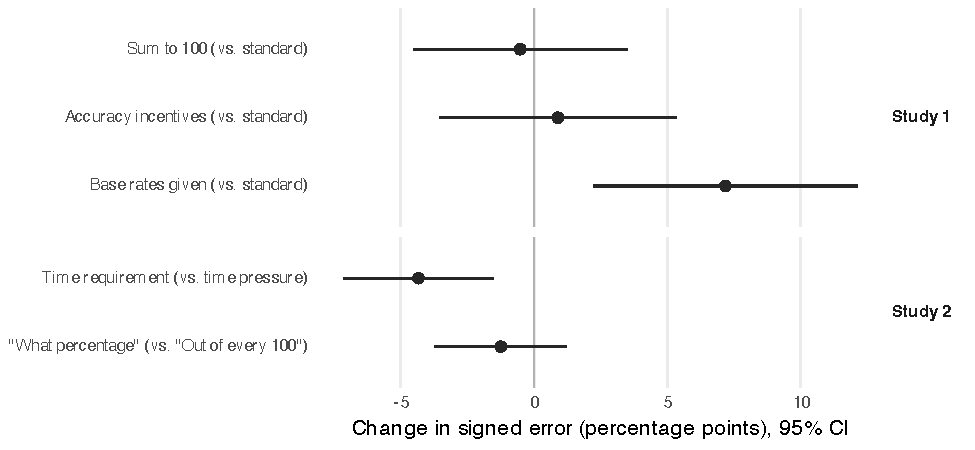
\includegraphics[width=\linewidth]{effects.pdf}
\caption{Average effects on signed error of changing how perceptions are elicited. Each estimate comes from a regression of signed error on a treatment indicator with item fixed effects; intervals use standard errors clustered by respondent. Positive values mean larger overestimates.}
\label{fig:effects}
\end{figure}

\subsection{Thinking fast and slow}

For all \timeItemsLower{} items in the timing experiment, the average answer was lower, and so less biased, in the time-requirement condition, although for the share of the poor who are Black the difference is just \timePoorDiff{} points. Item by item, \timeItemsFive{} differences are significant at $p<0.05$ and \timeItemsTen{} at $p<0.1$. Pooling across items, signed error was \timeEffect{} points lower with the time requirement (95\% CI \timeLo{} to \timeHi{}): \fastBias{} points under time pressure against \slowBias{} with the time requirement, a decline of about \timeDecline\%. Absolute error fell by \absTimeEffect{} points (Table~\ref{tab:alt}).

Respondents who had to wait might have used the time to look answers up. If they did, answers in the time-requirement condition should pile up at the truth. Figure~\ref{fig:density} shows no such spike. Counting answers that land on either whole number bracketing the truth, among the items each respondent saw, \noseSlow\% of answers in the time-requirement condition and \noseFast\% under time pressure were on the nose (difference \noseDiff{} points, $p=\noseP$; Table~\ref{tab:nose}). Even if every extra correct answer came from a lookup, lookups could account for less than half a point of the \timeEffect-point decline.

\subsection{Denominators larger than 100}

If people used denominators larger than 100, answers in the sum-to-100 condition should be lower. On average they were not: signed error was \standardBias{} points under standard estimation and \sumBias{} with the constraint, a difference of \sumEffect{} points. The average hides offsetting item effects (Figure~\ref{fig:items1}). The constraint lowered the estimated share of Democrats who are Black by \sumBlackAbs{} points. It raised the estimated share of Republicans who are Southern by \sumSouth{} points, from \standardSouthMean\% to \sumSouthMean\%, the largest item effect in either study. That item's complement had a single category, non-Southerners, so the constraint asked only for a split between two groups; why that raised the estimates is not clear from these data. The distribution tests in Table~\ref{tab:ks} tell the same story: only the Southern item differs at the 5\% level after adjusting for multiple tests.

Changing the wording yields similar results. Pooling across items, ``What percentage'' produced \wordEffect{} points less signed error than ``Out of every 100'' (95\% CI \wordLo{} to \wordHi): \percentBias{} points against \hundredBias. ``Out of every 100'' lowered estimates for only \hundredLowerItems{} of the ten items. It did lower the estimated foreign-born share, by \wordImm{} points, as \citet{sides2007b} would predict, but it raised the estimated share of Democrats who are gay, lesbian, or bisexual by \wordLgb{} points. Neither constraining respondents to the right denominator nor making it salient reduces bias on average.

\subsection{Motivated responding}

If motivated responding inflated the estimates, paying for accuracy should lower them. It did not: signed error was \incEffect{} points higher with incentives (95\% CI \incLo{} to \incHi), and the distribution of answers was similar on every item (Table~\ref{tab:ks}).

A separate MTurk survey from April 2014 \citep{ahler2018} offers observational evidence. Respondents rated the eight groups on 101-point feeling thermometers and later estimated the groups' shares in the party they do not identify or lean with. If dislike drove the estimates, colder ratings of a group should go with higher estimates of its share in the other party. Across groups, a one-point warmer rating went with a \thermoPooled-point lower estimate (95\% CI \thermoLo{} to \thermoHi; \thermoN{} respondents), and no group shows a relationship distinguishable from zero (Table~\ref{tab:thermo}).

\subsection{Beliefs about related quantities}

Valid reports can still be hard to interpret. In Study~1 respondents overestimated the population share of every party-stereotypical group, most of all for small groups. Gay, lesbian, and bisexual Americans are \lgbBaseTrue\% of adults in the 2012 ANES; respondents put them at \lgbBasePerceived\%. People earning more than \$250,000 a year are \richBaseTrue\%; respondents said \richBasePerceived\%. They put Black Americans at \blackBasePerceived\%, against \blackBaseTrue\%, consistent with \citet{wong2007}.

Respondents also put each group's share in its associated party above their own estimate of its population share (Table~\ref{tab:baserates}). The difference is significant at $p<0.05$ for \gapSigCount{} of the eight groups; it is not for Black Democrats or for atheist and agnostic Democrats. The difference-in-differences asks whether people overestimate a group's share in the party by more than they overestimate its share in the population:
\[
\bigl(\text{perceived}_{\text{party}} - \text{true}_{\text{party}}\bigr) - \bigl(\text{perceived}_{\text{population}} - \text{true}_{\text{population}}\bigr).
\]
A positive value means the error is concentrated in the party estimate, implicating party stereotypes rather than a misjudged base rate. The estimate is significantly positive for \ddPosCount{} of the eight groups and significantly negative for \ddNegCount. For Black Democrats it is \ddBlack{} (95\% CI \ddBlackLo{} to \ddBlackHi): respondents overestimate the Black share of the population by more than the Black share of Democrats, though the difference is not significant at the 5\% level.

The base-rates experiment gives a cleaner test. If ignorance of base rates drove the overestimates, starting the sliders at the base rate should lower them. Instead, signed error rose by \brEffect{} points (95\% CI \brLo{} to \brHi), and estimates rose for \brItemsUp{} of the eight items. Two readings fit. Respondents may neglect base rates, judging party composition by how typical a trait is of the party. Or they may infer that a researcher who shows them the population share expects the party share to differ from it, and adjust upward from the anchor. The experiment cannot separate the two, but either way, supplying base rates does not reduce bias.

Asking for a base rate first did not help in the diet-soda experiment either. Respondents not asked about the base rate put the share of women who drink diet soda at \sodaNoWomen\% and of men at \sodaNoMen\%, a gap of \sodaNoGap{} points against a true gap of about one point. Those asked first about all Americans (average estimate \sodaYesBase\%) put women at \sodaYesWomen\% and men at \sodaYesMen\%, a gap of \sodaYesGap{} points. The difference in gaps, \sodaDiff{} points (95\% CI \sodaLo{} to \sodaHi), is not statistically significant, but it points the same way as Study~1: prompting or supplying base rates did not reduce the bias and may have increased it.

\section{Conclusion}

Several politically important attitudes are linked to misperceptions of group size. Nativism is associated with overestimates of the immigrant population \citep{alba2005}, opposition to welfare with overestimates of the share of the poor who are Black \citep{gilens1996, gilens1999}, and partisan animus with overestimates of party-stereotypical groups in the other party \citep{ahler2018}. Campaigns exploit these beliefs; in 2016 both the Brexit campaign and Donald Trump's presidential campaign made claims about immigration levels central. Studying them requires valid measures.

For the items studied here, the experiments suggest that people hold beliefs about the size of salient, stereotyped groups and that numerical survey questions elicit them. Requiring answers to sum to 100, asking ``Out of every 100,'' and paying for accuracy did not change the average error, though the first two moved individual items in both directions. Considered answers were about a fifth less biased than rushed ones, with little sign that the extra time was used to look answers up. Supplying or prompting base rates did not reduce bias and may have increased it.

These conclusions may not hold for other items. We studied groups tied to prevalent stereotypes, about which people are more likely to hold crude but firm beliefs. Nor do the results rule out every concern for every measure here. Their use is to show how researchers can test the most pressing concerns in their own data.

\section*{Note on this version}

This version corrects the chapter published in \emph{Misinformation and Mass Audiences} \citep{ahlersood2018chapter}. The share of the poor who are Black is 23\% rather than 24.5\%, and the foreign-born share uses the 2014 rather than the 2010 American Community Survey. The ``What percentage'' baseline was misreported; it is \percentBias{} points rather than 18.9. The test for looking answers up counted items respondents never saw as wrong answers. The difference-in-differences for Black Democrats had a coding error that reversed its sign, and the population base rates now come from the same survey and coding as the party shares. The sum-to-100 condition sharply raised estimates of the Southern share of Republicans, which the chapter did not report. Study~1 had four conditions, not five. The interpretation of the base-rates experiment now acknowledges that anchoring and conversational inference also fit the result.

\bibliographystyle{apsr}
\bibliography{references}

\clearpage
\appendix
\renewcommand{\thetable}{A\arabic{table}}
\renewcommand{\thefigure}{A\arabic{figure}}
\setcounter{table}{0}
\setcounter{figure}{0}

\section{Appendix}

\begin{table}[htbp]
\centering
\caption{Sample composition (\%). Study~1 race is check-all-that-apply; Study~2 offered one choice. Study~2 did not ask about education.}
\label{tab:samples}
{\TableStyle\begin{tabular}{lrr}
\toprule
  & Study 1 (2014) & Study 2 (2016) \\
\midrule
\multicolumn{3}{l}{\emph{Party}} \\
Democrat (incl. leaners) & 58.9 & 55.0 \\
Republican (incl. leaners) & 18.8 & 27.9 \\
Independent & 22.3 & 17.1 \\
\addlinespace
\multicolumn{3}{l}{\emph{Gender}} \\
Female & 50.5 & 50.6 \\
Male & 49.5 & 49.4 \\
\addlinespace
\multicolumn{3}{l}{\emph{Race and ethnicity}} \\
White & 76.2 & 76.5 \\
Black & 8.1 & 7.1 \\
Asian & 9.4 & 9.1 \\
Latino & 9.7 & 5.4 \\
\addlinespace
\multicolumn{3}{l}{\emph{Education}} \\
Less than high school & 0.5 & -- \\
High school & 9.7 & -- \\
Some college & 46.1 & -- \\
4-year degree & 34.8 & -- \\
Advanced degree & 8.9 & -- \\
\addlinespace
\multicolumn{3}{l}{\emph{Age}} \\
18-39 & 79.1 & 65.4 \\
40-64 & 19.1 & 32.0 \\
65+ & 1.8 & 2.5 \\
\bottomrule
\end{tabular}
}
\end{table}

\begin{table}[htbp]
\centering
\caption{Benchmarks. True shares for the party items are among identifiers and leaners. Population base rates are the groups' shares among all adults, from the same source.}
\label{tab:benchmarks}
{\TableStyle\begin{tabular}{lrr}
\toprule
Item & True share & Population base rate \\
\midrule
Dem. black & 24.0 & 12.9 \\
Dem. LGB & 6.3 & 3.9 \\
Dem. union & 10.5 & 9.2 \\
Rep. \$250K+ & 2.2 & 1.7 \\
Rep. Southern & 35.7 & 33.6 \\
Rep. 65+ & 21.3 & 18.9 \\
Dem. atheist/agnostic & 8.7 & 5.7 \\
Rep. evangelical & 34.3 & 19.0 \\
U.S. foreign-born & 13.2 & -- \\
Poor who are black & 23.1 & -- \\
\bottomrule
\end{tabular}
}
\end{table}

\begin{figure}[htbp]
\centering
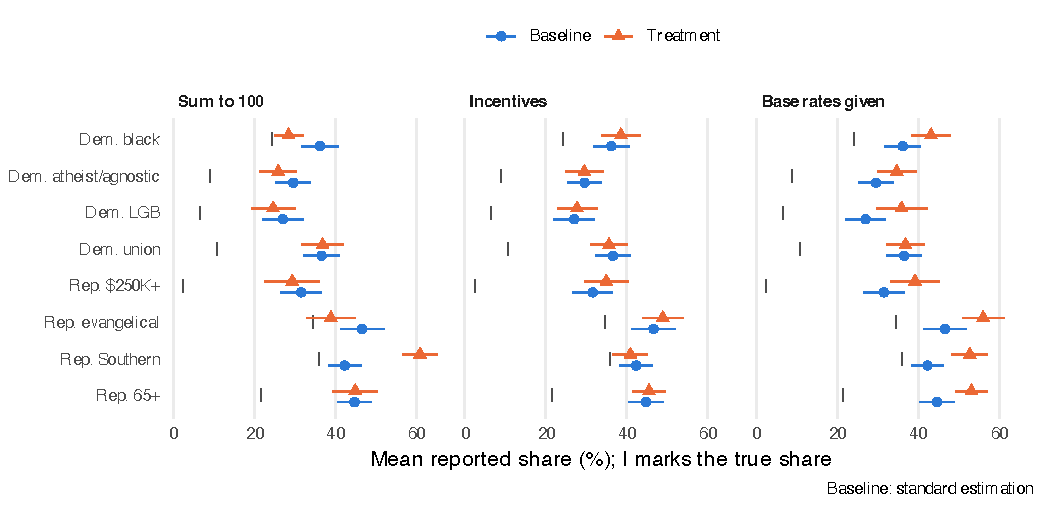
\includegraphics[width=\linewidth]{items_study1.pdf}
\caption{Study~1: mean reported share by item and condition, with 95\% intervals. Each panel compares one condition with standard estimation.}
\label{fig:items1}
\end{figure}

\begin{figure}[htbp]
\centering
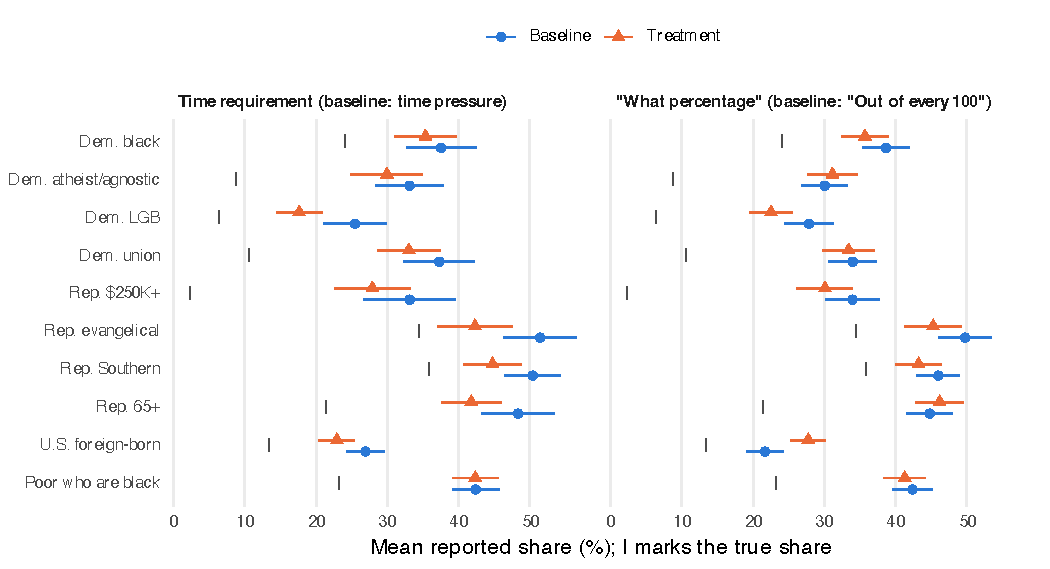
\includegraphics[width=\linewidth]{items_study2.pdf}
\caption{Study~2: mean reported share by item and condition, with 95\% intervals.}
\label{fig:items2}
\end{figure}

\begin{table}[htbp]
\centering
\caption{Study~1: Kolmogorov--Smirnov tests comparing each condition's answers with standard estimation. Cells show the $D$ statistic and, in parentheses, the $p$-value adjusted for the eight tests in each column \citep{benjamini1995}.}
\label{tab:ks}
{\TableStyle\begin{tabular}{llll}
\toprule
Group & Sum to 100 & Incentives & Base rates given \\
\midrule
Dem. black & 0.20 (0.40) & 0.08 (0.98) & 0.23 (0.08) \\
Dem. atheist/agnostic & 0.11 (0.97) & 0.14 (0.98) & 0.17 (0.16) \\
Dem. LGB & 0.09 (0.97) & 0.10 (0.98) & 0.19 (0.11) \\
Dem. union & 0.11 (0.97) & 0.09 (0.98) & 0.09 (0.78) \\
Rep. \$250K+ & 0.09 (0.97) & 0.11 (0.98) & 0.18 (0.11) \\
Rep. evangelical & 0.21 (0.37) & 0.12 (0.98) & 0.20 (0.11) \\
Rep. Southern & 0.49 (0.00) & 0.07 (0.98) & 0.19 (0.11) \\
Rep. 65+ & 0.11 (0.97) & 0.07 (0.98) & 0.19 (0.11) \\
\bottomrule
\end{tabular}
}
\end{table}

\begin{table}[htbp]
\centering
\caption{Pooled effects on alternative outcomes. Absolute error is the distance from the true share; percentage bias is signed error as a percentage of the true share. Regressions include item fixed effects; standard errors are clustered by respondent. * $p<0.1$, ** $p<0.05$, *** $p<0.01$.}
\label{tab:alt}
\adjustbox{max width=\linewidth}{\TableStyle
\begin{tabular}{llrrrrr}
\toprule
Outcome & Comparison & Baseline & Effect & SE & Answers & Respondents\\
\midrule
Signed error & Time requirement & 19.8 & -4.3*** & 1.4 & 1696 & 284\\
Signed error & Percent wording & 19.1 & -1.2 & 1.3 & 3119 & 312\\
Absolute error & Time requirement & 22.0 & -3.5*** & 1.2 & 1696 & 284\\
Absolute error & Percent wording & 22.3 & -1.1 & 1.1 & 3119 & 312\\
Percentage bias & Time requirement & 228.3 & -48.1** & 20.2 & 1696 & 284\\
Percentage bias & Percent wording & 269.4 & -23.9 & 18.0 & 3119 & 312\\
\bottomrule
\end{tabular}
}
\end{table}

\begin{figure}[htbp]
\centering
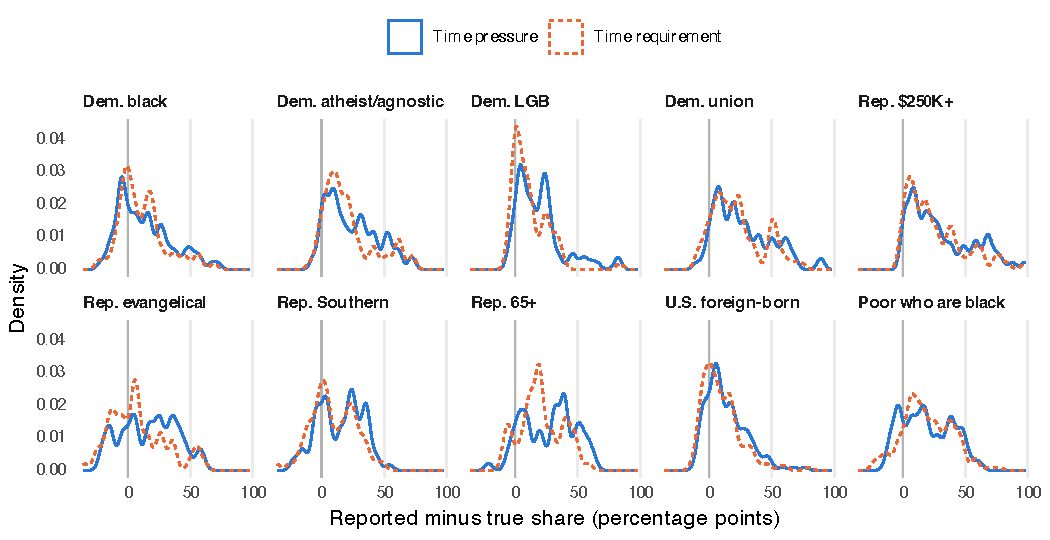
\includegraphics[width=\linewidth]{timing_density.pdf}
\caption{Timing experiment: distribution of answers relative to the true share. Looking answers up would show as a spike at zero in the time-requirement condition.}
\label{fig:density}
\end{figure}

\begin{table}[htbp]
\centering
\caption{Timing experiment: percentage of answers on either whole number bracketing the true share, among the items each respondent saw. Item rows use Welch $t$-tests; the last row pools items with item fixed effects and respondent-clustered standard errors.}
\label{tab:nose}
{\TableStyle
\begin{tabular}{lrrrrr}
\toprule
Item & Time pressure & Time requirement & Difference & 95\% CI & p\\
\midrule
Dem. black & 2.7 & 4.2 & 1.5 & {}[-4.5, 7.5] & 0.62\\
Dem. atheist/agnostic & 4.3 & 1.6 & -2.7 & {}[-8.5, 3.1] & 0.36\\
Dem. LGB & 4.2 & 10.5 & 6.4 & {}[-2.1, 14.8] & 0.14\\
Dem. union & 3.8 & 6.1 & 2.3 & {}[-4.5, 9.1] & 0.50\\
Rep. \$250K+ & 4.9 & 1.4 & -3.5 & {}[-9.7, 2.6] & 0.26\\
Rep. evangelical & 4.2 & 5.9 & 1.7 & {}[-5.8, 9.1] & 0.66\\
Rep. Southern & 2.6 & 9.9 & 7.3 & {}[-0.7, 15.2] & 0.07\\
Rep. 65+ & 1.6 & 0.0 & -1.6 & {}[-4.9, 1.6] & 0.32\\
U.S. foreign-born & 3.6 & 7.7 & 4.1 & {}[-1.3, 9.6] & 0.13\\
Poor who are black & 1.4 & 2.1 & 0.7 & {}[-2.4, 3.8] & 0.67\\
All items (item fixed effects) & 3.2 & 5.0 & 1.9 & {}[-0.1, 3.9] & 0.07\\
\bottomrule
\end{tabular}
}
\end{table}

\begin{table}[htbp]
\centering
\caption{Study~1, standard estimation: perceived population base rates and party shares among respondents asked both. ``Party - base'' is perceived party share minus perceived base rate; the difference-in-differences subtracts the error in the base rate from the error in the party share. Both are computed within respondent. * $p<0.1$, ** $p<0.05$, *** $p<0.01$.}
\label{tab:baserates}
\adjustbox{max width=\linewidth}{\TableStyle\begin{tabular}{lrrrrrrrr}
\toprule
Group & n & Base, true & Base, perceived & Party, true & Party, perceived & Party - base & DiD & DiD 95\% CI \\
\midrule
Dem. black & 45 & 12.9 & 31.4 & 24.0 & 36.0 & 4.6 & -6.5* & [-14.2, 1.3] \\
Dem. atheist/agnostic & 56 & 5.7 & 22.9 & 8.7 & 28.0 & 5.1* & 2.1 & [-3.3, 7.5] \\
Dem. LGB & 49 & 3.9 & 14.9 & 6.3 & 27.3 & 12.5*** & 10.1** & [1.5, 18.6] \\
Dem. union & 54 & 9.2 & 25.7 & 10.5 & 33.5 & 7.8*** & 6.5*** & [1.8, 11.2] \\
Rep. \$250K+ & 57 & 1.7 & 11.4 & 2.2 & 28.6 & 17.2*** & 16.7*** & [10.3, 23.2] \\
Rep. evangelical & 46 & 19.0 & 35.5 & 34.3 & 50.0 & 14.5*** & -0.8 & [-7.5, 5.8] \\
Rep. Southern & 35 & 33.6 & 32.7 & 35.7 & 41.9 & 9.2*** & 7.2** & [1.4, 13.0] \\
Rep. 65+ & 50 & 18.9 & 30.4 & 21.3 & 46.5 & 16.2*** & 13.7*** & [6.2, 21.3] \\
\bottomrule
\end{tabular}
}
\end{table}

\begin{table}[htbp]
\centering
\caption{April 2014 survey: regressions of the perceived share of each group in the other party on the respondent's feeling thermometer rating of the group, with HC2 standard errors. Republican respondents and independents estimated Democratic shares; Democrats and independents estimated Republican shares. ``Under 35'' replaced ``65 or older'' in this survey.}
\label{tab:thermo}
{\TableStyle
\begin{tabular}{lrrrr}
\toprule
Party and group & Coefficient & SE & 95\% CI & n\\
\midrule
Dem. black & -0.02 & 0.06 & {}[-0.13, 0.09] & 316\\
Dem. atheist/agnostic & -0.03 & 0.05 & {}[-0.13, 0.07] & 316\\
Dem. LGB & -0.06 & 0.05 & {}[-0.17, 0.05] & 316\\
Dem. union & -0.05 & 0.06 & {}[-0.17, 0.07] & 316\\
Rep. \$250K+ & 0.01 & 0.04 & {}[-0.08, 0.09] & 686\\
Rep. evangelical & -0.03 & 0.04 & {}[-0.10, 0.04] & 686\\
Rep. Southern & -0.03 & 0.03 & {}[-0.10, 0.04] & 686\\
Rep. under 35 & 0.02 & 0.03 & {}[-0.03, 0.07] & 686\\
\bottomrule
\end{tabular}
}
\end{table}

\begin{figure}[htbp]
\centering
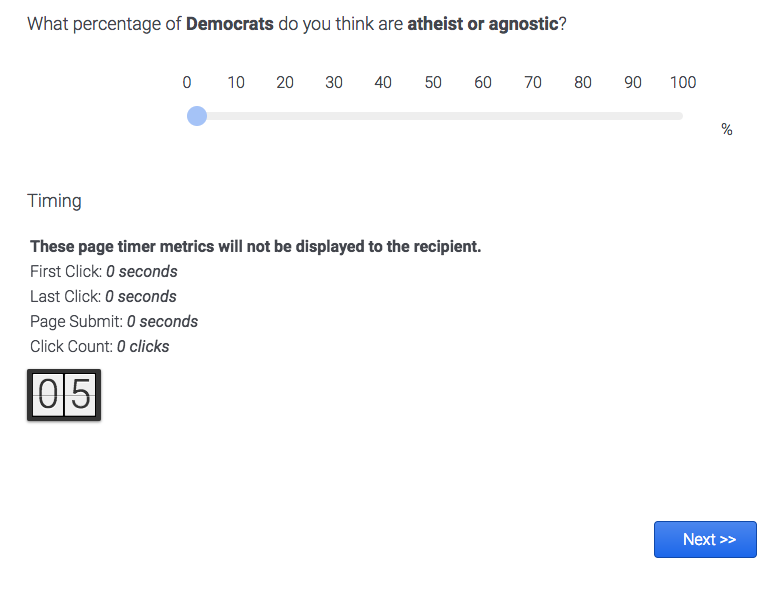
\includegraphics[width=0.48\linewidth]{study2_timing_fast.png}\hfill
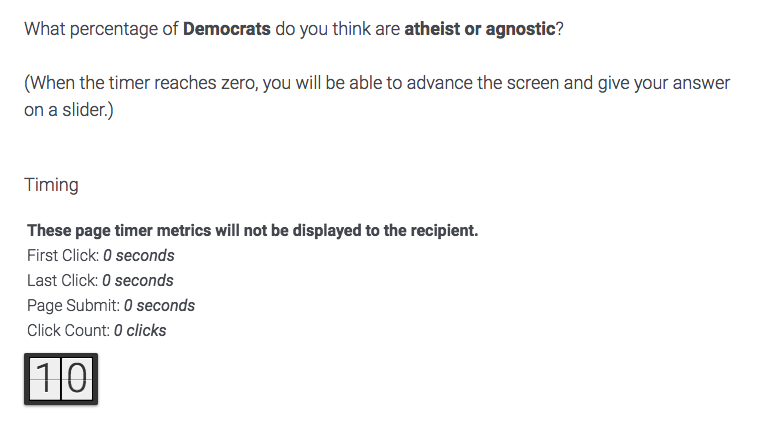
\includegraphics[width=0.48\linewidth]{study2_timing_slow.png}
\caption{Study~2 timing experiment: time pressure (left) and time requirement (right).}
\end{figure}

\begin{figure}[htbp]
\centering
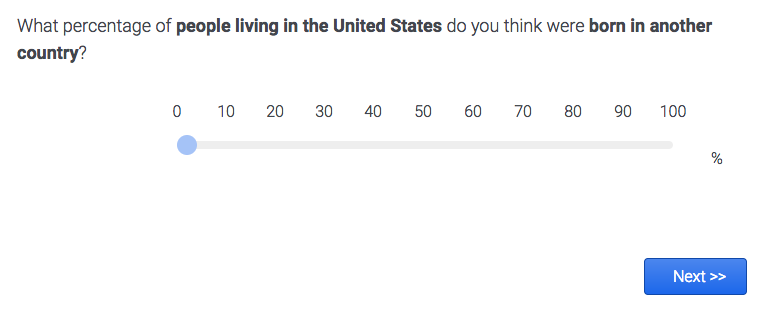
\includegraphics[width=0.48\linewidth]{study2_wording_perc.png}\hfill
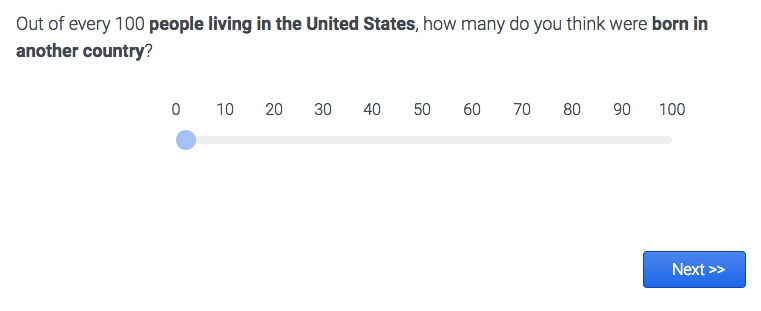
\includegraphics[width=0.48\linewidth]{study2_wording_hundred.png}
\caption{Study~2 wording experiment: ``What percentage'' (left) and ``Out of every 100'' (right).}
\end{figure}

\begin{figure}[htbp]
\centering
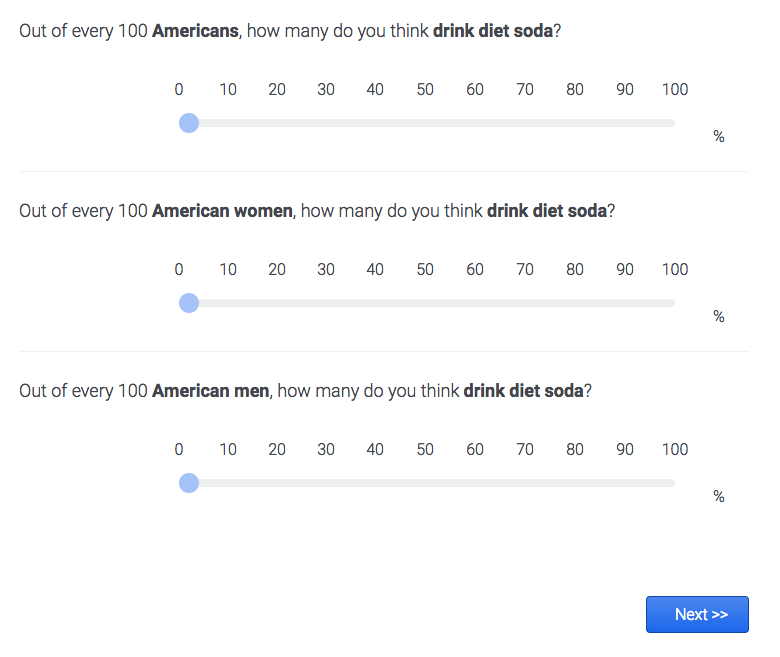
\includegraphics[width=0.6\linewidth]{study2_soda.png}
\caption{Study~2 diet-soda items. Respondents in the control condition did not see the first item.}
\end{figure}

\end{document}
